\chapter[EXEMPLO DE USO]{EXEMPLO DE USO}
\label{chapter:example}

Como forma de ilustração de uso do serviço que desenvolvemos elaboramos uma
aplicação que chamamos de Forensic, que interage com o Shock via Kafka,
respeitando as definições feitas à cerca da API. A aplicação foi feita em
Elixir, uma linguagem funcional desenhada para construir aplicações
manuteníveis e escaláveis, utilizando o \textit{framework} Phoenix, que
facilita no desenvolvimento de aplicações Web.

O Forensic tem como principais objetivos abstrair o Shock do usuário final,
e consequentemente, as ferramentas de Big Data (como o Spark), ao passo em que
fornece um conjunto de funcionalidades que permitem ao usuário final configurar
a atuação dos \textit{streams}, semelhante a outros serviços existentes,
como o Amazon AWS\footnote{\url{https://aws.amazon.com/kinesis/analytics/}}.
Um usuário que deseje interagir com o Shock e o InterSCity deve
(i) configurar um \textit{stream} novo com os
parâmetros desejados; (ii) criar esse \textit{stream} no Shock; (iii) injetar
esse \textit{stream} no Shock; (iv) e iniciar o processamento do
\textit{stream}. O Forensic então abstrai esses 4 passos, facilitando o uso
das ferramentas e da plataforma.

Do ponto de vista da implementação, o Forensic espelha as abstrações do Shock
(como os \textit{streams}) e apresenta outras. Um dos conceitos necessários para seu
uso efetivo é o entendimento da arquitetura de camadas
\textit{ingest, store, analyze} e \textit{publish}, apresentada na Figura
\ref{fig:ingeststore}, que criamos para o Forensic. Essa arquitetura é baseada
em arquiteturas mais difundidas, como a \textit{ingest, store, analyze} e
\textit{visualize}, utilizada na plataforma Google Cloud
Platform\footnote{\url{https://cloud.google.com/solutions/data-lifecycle-cloud-platform}},
e a arquitetura \textit{collecton tier, message queuing tier, analysis tier,
in-memory data store} e \textit{data access tier}, explicada em
\citeonline{psaltis2017streaming}. O Forensic usa a abstração de \textit{stages}
para implementar a arquitetura mencionada, onde cada \textit{stage}
representa um passo da arquitetura. Um \textit{stream} tem no máximo
4 \textit{stages}, e caso um necessite de mais, novos \textit{streams} devem
ser criados, e o resultado de um \textit{stream} deve ser utilizado como entrada
em outro.

A API que o Shock fornece para comunicação se assemelha ao formato JSON, mas
via Kafka. Essa API espera mensagens no padrão ``arg1;\{arg2\}'',
onde o primeiro \textit{token} (antes do ponto e vírgula), ``arg1'', representa o nome
da ação desejada, e o segundo, ``arg2'', os argumentos da ação. Um
\textit{handler} no Shock receberá a ação requisitada no método
\textit{handle}, e deve tratar a requisição recebida. Por exemplo, uma mensagem
\small{\textbf{ingestion;\{"stream": "mystream", "shock\_action": "socketIngestion"\}}},
deve ser enviada caso queira-se o registro de um estágio de ingestão no
\textit{stream} \textit{mystream} utilizando a estratégia \textit{socketIngestion}.

\begin{figure}
  \centering
  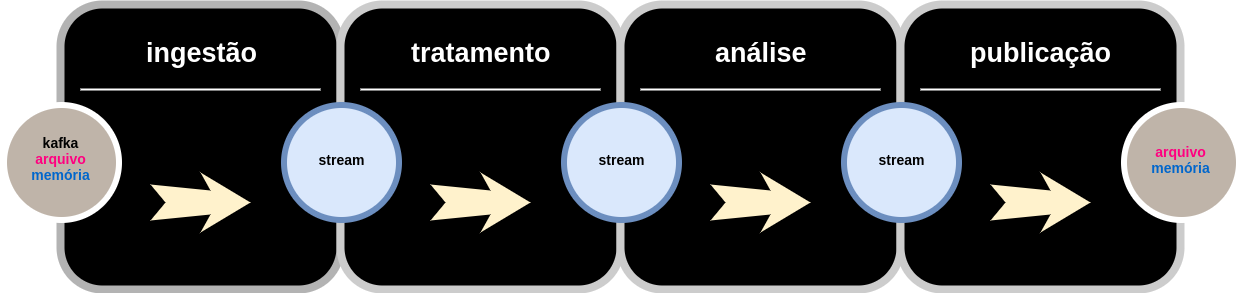
\includegraphics[width=\textwidth]{figuras/arquiteturaforensic.png}
  \caption{Padrão \textit{ingest, store, analyze e publish.}}
  \label{fig:ingeststore}
\end{figure}

O primeiro estágio de um \textit{stream}, \textit{\textbf{ingest}}, trata-se da
ingestão dos dados a partir de alguma fonte, como algum tópico do Kafka, ou
algum arquivo novo. Atualmente o Shock fornece três tipos diferentes de
ingestão: ingestão via tópico do Kafka, ingestão via arquivo (Parquet e JSON)
e ingestão via \textit{socket}. A depender da estratégia de ingestão, alguns
parâmetros são necessários na configuração - numa ingestão via Kafka, por
exemplo, é necessário configurar o endereço do
\textit{broker} e os tópicos que serão utilizados. Ao final, o Forensic deve
passar os parâmetros configurados para o Shock, que ajustará no Spark.
A Figura \ref{fig:forensicparams}
apresenta a página de configuração de um \textit{stream} no Forensic.

\lstinputlisting[float,floatplacement=H,caption={
  Ingestão de dados no Shock via \textit{socket} e Kafka.
  }]{editaveis/arquivos/ingestion.py}

\begin{figure}
  \centering
  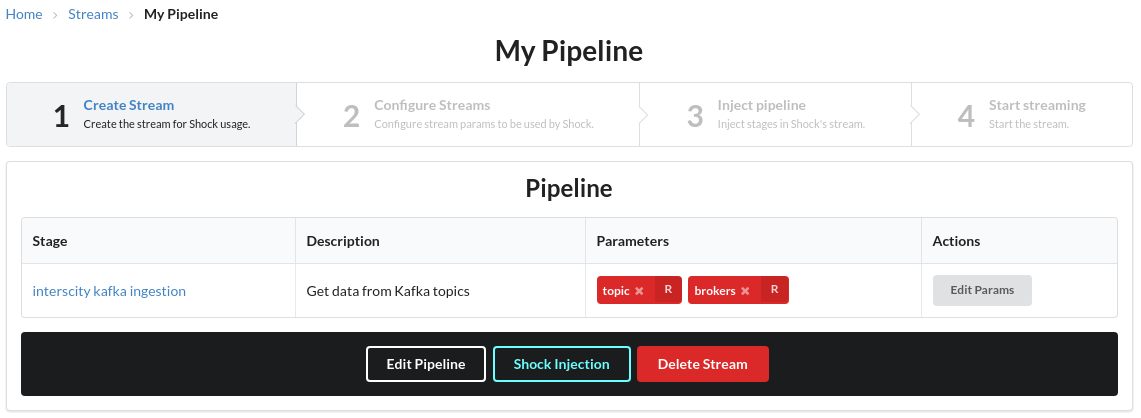
\includegraphics[width=\textwidth]{figuras/pipeline.png}
    \caption{Página de configuração de um \textit{stream}. Os parâmetros
obrigatórios (\textit{topic e brokers}) foram configurados.}
  \label{fig:forensicparams}
\end{figure}

O segundo estágio de um \textit{stream}, \textit{\textbf{store}}, recebe no
Forensic um papel diferente do sugerido pela literatura. No Forensic
ele não trata somente de um estágio de armazenamento de dados, mas sim de um
estágio de \textit{setup}, podendo ser feita a limpeza dos dados. Um
exemplo típico é o uso de um estágio de \textit{store} que faça \textit{cast}
de dados, quando valores estão como \textit{string} quando são necessários valores
\textit{double}. O Shock apresenta somente \textit{stores} de \textit{cast},
que são essenciais no uso do InterSCity e de consumo do Kafka.

\lstinputlisting[float,floatplacement=H,caption={
  Tratamento de dados no Shock via \textit{cast}.
}]{editaveis/arquivos/store.py}

O terceiro estágio de um \textit{stream}, \textit{\textbf{analyze}}, é o
estágio principal do processamento, e permite filtros, agregações e cálculos.
No Shock, a etapa de análise dos dados recebe como entrada um \textit{stream}
de dados e devolve um \textit{stream} transformado. Uma aplicação que deseje
utilizar a operação de filtro no \textit{stream} \textit{mystream} com a finalidade
de filtrar os valores de \textit{air\_quality} iguais a 31, deve fazer uma
requisição no Kafka com o conteúdo \small{\textbf{processing;\{"stream": "mystream",
"shock\_action": "streamFilter", "query": "select * from air\_quality where
'value' == 31"\}}}, ou configurar via Forensic.

\lstinputlisting[float,floatplacement=H,caption={
  Operações de análise de dados no Shock.
}]{editaveis/arquivos/processing.py}

O último estágio de um \textit{stream}, \textit{\textbf{publish}}, é o estágio
de apuração do processamento, retornando os dados necessários para o cliente.
O Shock atualmente permite a publicação via arquivo, memória e console, e após o
lançamento da versão 2.2 do Spark, permitirá a publicação via Kafka. A
publicação via arquivo é limitada, pois não permite a publicação em um servidor
externo. A publicação via memória também não permite, mas é interessante pois
o conteúdo passa a estar disponível para ser requisitado via SparkSession,
permitindo consultas com síntaxe SQL. Por fim, a publicação via \textit{console} está
presente somente para fins de desenvolvimento, mas é possível que ocorra uma
combinação com outras ferramentas que leiam da saída padrão. Categorizamos
no Shock o nome \textit{sink} para as diferentes estratégias de publicação,
que é o nome utilizado pelo Spark.

\lstinputlisting[float,floatplacement=H,caption={
  Estratégias de publicação de resultados presentes no Shock.
}]{editaveis/arquivos/sinks.py}

Como alternativa às limitações de publicação dos dados, o Shock disponibiliza
na API os \textit{flushes}, que atuam como um \textit{job} adicional que ingere
dados de alguma fonte (que não seja um \textit{stream}) e publica em outra.
Como estudo de caso para o InterSCity, estamos utilizando \textit{flushes} que
recebem como entrada consultas no SparkSession (que foi populado pela
publicação via memória), e que publicam em uma fonte desejada via
\textit{websocket}. Essa alternativa não precisaria existir caso
a publicação via Kafka já estivesse disponível no Spark, mas enquanto o
lançamento da versão 2.2 não ocorre, acaba sendo uma opção válida.

Com o propósito de aproximar cenários mais reais às desenvolvidas, separamos
três casos de uso para uso no Forensic e no Shock, utilizando como bases alguns
coletores de dados de São
Paulo\footnote{\url{https://github.com/lucaskanashiro/collect_sp_data}}. De
maneira geral, os casos de uso abrangem todos os conceitos e estágios citados
anteriormente, como o \textit{cast} de dados, filtros, dentre outros.

\section{CASO DE USO 1 - REGIÕES COM QUALIDADE DO AR INSATISFATÓRIA}

O primeiro caso que separamos é o de regiões que apresentam qualidade do ar
insatisfatória, utilizando como base os dados da
CETESB\footnote{\url{http://sistemasinter.cetesb.sp.gov.br/Ar/php/ar_resumo_hora.php}}.
A solução desse caso de uso pode ser divida em três etapas:
\begin{enumerate}
    \item Coletar os dados;
    \item Publicar os dados no InterSCity;
    \item Configurar um \textit{stream} que filtre os dados, removendo
        da lista os dados com boa qualidade do ar (pois queremos as regiões
        com qualidade insatisfatória).
\end{enumerate}

O primeiro passo, de coleta dos dados, pode ser resolvido via \textit{crawler},
para extrair e normalizar os dados do \textit{site}. Um \textit{script} que
utiliza o Mechanize já havia sido desenvolvido por contribuidores do
InterSCity\footnote{\url{https://github.com/lucaskanashiro/collect_sp_data/blob/master/air_quality.rb}},
e pôde ser reaproveitado.

O segundo passo, de publicação dos dados no InterSCity, se baseia na
normalização dos dados e das requisições, para que aja uma interação com o
Resource Adaptor. Adaptamos o \textit{script} mencionado no passo anterior
para que passasse a fazer requisições REST ao Resource Adaptor do InterSCity,
possibilitando o registro de recursos e o envio dos dados.

O terceiro passo, de configuração do \textit{stream}, é feito através do Forensic.
Um \textit{stream} deve ser criado na interface, e configurado para uso dos
\textit{stages} \textit{Kafka Ingestion}, \textit{Kafka Cast} e \textit{Filter}.
O quarto \textit{stage}, de \textit{publish}, é mais flexível, e qualquer
estratégia disponível no Forensic serve para esse caso de uso. O Forensic
apresenta uma página de alertas, que é populada via um \textit{flush}
específico. Quando esse \textit{flush} é acionado, o Shock organiza um \textit{job}
que lê de um repositório específico no formato Parquet, e publica no Forensic
os dados via \textit{websocket}.

\lstinputlisting[float,floatplacement=H,language=elixir,caption={Consumo dos dados via \textit{websocket}
caso o evento seja \textit{new\_event}.}]{editaveis/arquivos/channel.ex}

Após o \textit{stream} ser criado e os \textit{stages} selecionados, basta
configurar os parâmetros e transferir as definições para o Shock. A Figura
\ref{fig:case1} apresenta uma tela do Forensic com os \textit{stages}
mencionados selecionados. Para os \textit{stages} utilizados, as
configurações de parâmetros foram:

\begin{itemize}
    \item \textbf{Kafka Ingestion:} O parâmetro \textit{topic} foi definido
        como \textit{interscity}, e é o tópico onde o InterSCity publica
        novos dados. O parâmetro \textit{brokers} foi definido como
        \textit{kafka:9092}, referente ao endereço do Kafka no contêiner do
        Docker utilizado para esse exemplo;
    \item \textbf{Kafka Cast:} Esse \textit{stage} não precisa ser configurado.
    \item \textbf{Filter:} O parâmetro \textit{query} desse filtro foi
        configurado com o valor \textit{capability == `air\_quality` AND value != `Boa`},
        filtrando \textit{capabilities} que não são sobre qualidade do ar e
        com valores não satisfatórios;
    \item \textbf{Parquet Publishing:} O parâmetro \textit{path} foi definido
        como \textit{/analysis}, que será utilizado pelo \textit{flush} como
        mencionado anteriormente.
\end{itemize}

\begin{figure}
  \centering
  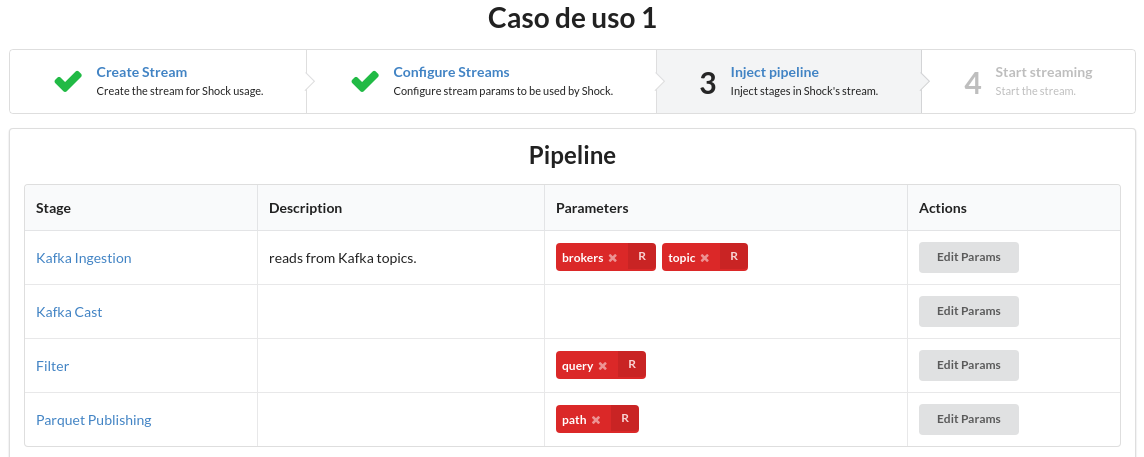
\includegraphics[width=\textwidth]{figuras/parametros.png}
  \caption{Parâmetros do primeiro caso.}
  \label{fig:case1}
\end{figure}

